\chapter{Arhitektuur}
\section{Arhitektuuri ajaloost}
Inimesed on aastatuhandeid maju ehitanud. Ja sama vana on arhietkuuri mõiste. Ka meie esivanematel oli väga selge ettekujutus, kui suur üks hea rehetare peaks olema, mis ilmakaarde vaatama ning kuidas paiknema vee suhtes. Mis see muu on, kui arhitektuur?

\begin{marginfigure}
	\begin{center}
		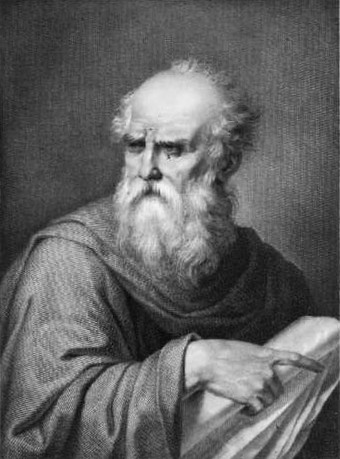
\includegraphics[width=.84\linewidth]{vitruvio.jpg}
		\caption{Marcus Vitruvius Pollio, 80-70 eKr.- 15 pKr}
		\label{fig:vitruvius}
	\end{center}
\end{marginfigure}

Siinkandis\sidenote{Induse orus tekkisid linnastud juba 2600 e.k., ilmselt tegeldi seal ka arhitektuuriga} ehk kõige kuulsamad majaehitajad olid kreeklased. Rooma impeeriumi laienemisega oli kõikjale vaja luua uusi asundusi ja kindlustatud tugipunkte. Seega oli suur vajadus ka arhitektide järele. Meie ajaarvamise alguse Rooma riigist pärinebki ehk esimene terviklik kästilus arhitektuurist\cite{pollio1914vitruvius}. 

Too Vitruviuse teos on tänaseni märkimisväärselt loetav ja aktuaalne. Samm-sammult kirjeldatakse eritüübiliste hoonete planeerimise ja konstrueerimise detaile alates üldisetest põhimõtetest (Alati ehita linna peatänav risti talviste tuulte peamise suunaga) kuni sammaste täpsete mõõtmeteni. Sellisena on tegemist tavapärasest arhitektuurist oluliselt laiema kandepinnaga teosega. Rõhk kasutaja vajadustel, juhised konteksti arvestamiseks ning tugev seos insenerikunstiga on kõik asjad, mis on tänasele tarkvaraarhitektile täpselt sama olulised kui toonasele majaehitejale. 

Ehk kõige olulisem Vitruviuse pärand on tema kolm üldist printsiipi, millele kõik ruumiga tegelevad kunstid alluma peaksid\index{Arhitektuur!Printsiibid}: tugevus (püsivus), otstarbekus, ilu.\cite{vitruviusest}. Tol ajal arvuteid polnud kuid samade printsiipide rakenduvuse vastu tänapäevases tarkvara arhitektuuris on raske vaielda. 

Viimase paarisaja aasta jooksul on arhitektuurimõte küll edasi arenenud, kuid, huvitaval kombel, ei ole esile kerkinud ühtset arhitektuuri definitsiooni. Enamasti mõeldakse arhikektuuri all millegi osiste ning nende seoste skemaatilist kirjeldust. Selline lähenemine on aga piiratud, sest räägib vähe tolle kirjelduse tekkeprotsessist või ka arhitektuuri kui sellise väärtusest. Läheb kaotsi arhitekti töö loominguline komponent. Samuti on nii mõeldes lihtne takerduda valdkondade piiridesse: arhitektuuridokumente toodetakse ju eesmärgiga ühe või teise elukutse esindajale juhiseid anda. Aga kuhu jääb tervik? 

IT strateegia kontekstis on tüüpiliselt objektiks, mida disainida, organisatsiooni tegevust toetav infosüsteem. Et sedalaadi infosüsteemide disain on olulise ärilise tähendusega, on arenenud terve tarkvara arhitektuuri haru, ettevõttearhitektuur\sidenote{Ingl. \emph{Enterprise Architecture}. Tegemist on mõnevõrra eksitava mõistega, kuna tüüpiliselt on tähelepanu ettevõtte infosüsteemide ja mitte ettevõtte kui sellise arhitektuuril}.

\section{Paradigmamuutus ettevõttearhitektuuris}
\label{sec:architecture:paradigm}
Ettevõtte arhitektuuriraamistike\index{EA} ajalugu algab 1987. aastal Zachmani klassikalise paberiga \cite{zachman1987framework}. Sellest alates on toimunud päris oluline areng, mille üldjoontes võtab kokku joonis \ref{fig:architecture:EA}. 

\begin{figure}%
	\begin{center}
		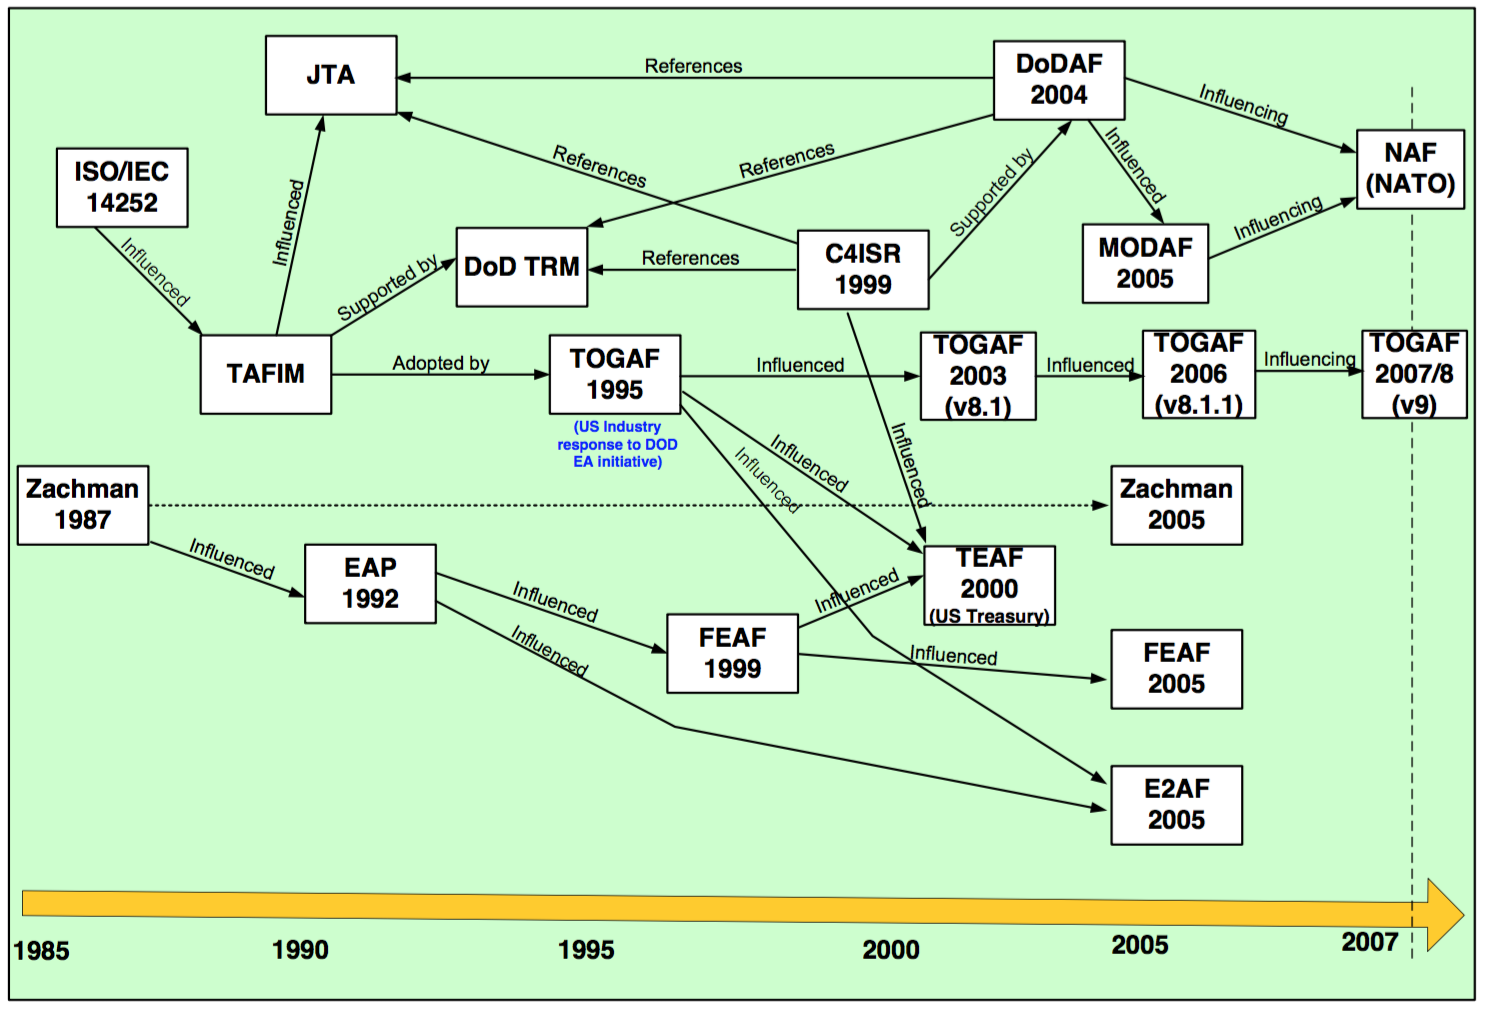
\includegraphics[width=\linewidth]{eaevolution.png}
		\caption{Arhitektuuriraamistike evolutsiooniline kontekst}
		\label{fig:architecture:EA}
	\end{center}
\end{figure}

Siit paistab nii mõndagi huvitavat. Kõigepealt on näha, et raamistikud uuenevad jämedalt viie-aastase kadentsiga. Teiseks on märgatav militaarorganisatsioonide oluline mõju. Kolmandaks näeme, et joonis lõpeb aastaga 2007. 2009. aastal on üllitatud küll DoDAF\index{DoDAF} v. 2.02 aastal 2010 kuid isegi raamistikke võrdlevat kirjandust on sel kümnendil ilmunud vähe. Siit võib järeldada, et ühel või teisel põhjusel liiguvad arhitektuuriraamistikud tehnoloogia arengust oluliselt aeglasemalt ning et valdkond on teatavas mõttes kriisis. Tõenäoliselt saavad üksikud spetsiifiliste vajadustega organisatsioonid nagu NATO või USA kaitseministeerium oma raamistikest väärtust, kuid nende rakendatavus väljaspool militaarvaldkonda on küsitav. 

Põhjusi on ilmselt mitmeid, kuid tõenäoliselt on oma roll nii organisatsioonide kui nende keskkonna keerukuse kasvul. Võib välja tuua neli eeldust, mis raamistike kuldajal sajandivahetuse paiku veel enamasti kehtisid kuid täna on tõesed järjest väiksema hulga ettevõttearhitektuurist kasu saada võivate organisatsioonide puhul.

\textbf{Organisatsioonid on kultuuriliselt, tehniliselt jne. homogeensed}. Isegi, kui tegu oli rahvusvaheliste organisatsioonidega, ei pruukinud eraldiseisvad üksused olla tihedalt integreeritud. Integratsioon eeldab kommunikatsiooni ja seda on ilma internetita keeruline efektiivselt korraldada. \citeauthor{cfmcommnetworks}\cite{cfmcommnetworks} näitab, et keskmine teadmustöötaja USAs suhtles veel sajandivahetuse paiku isegi e-posti olemasolul vaid temast väga piiratud füüsilises raadiuses olevate inimestega. See tähendas, et mitmesuguseid kultuurilisi, tehnilisi vms. piire tuli igapäevases töös ületada suhteliselt harva. Tänapäeval on ka Eestis vähegi edukamate ettevõtete kliendid ja töötajad maailmas laiali ning meie sotsiaalsed, juriidilised ja ärilised suhted on üha enam piiriülesed\sidenote{Maailm tundub üha väiksemaks jäävat. Tavapäraselt arvatakse, et globaalse suhtevõrgustiku keskmine kaugus kahe inimese vahel on kuus. Facebook on leidnud selle numbri aastal 2015 olevat 3.57, sama number aastal 2011 oli 3.74\citep{backstrom2012four}}. Otsuste tegemisel ei saa enam eeldada, et otsuse täideviijat õnnestub efektiivselt mõjutada ning et tollel täideviijal, kui kohaliku konteksti tundjal, ei ole head põhjust otsuse vastu tõrkuda. Samuti on järjest ohtlikum eeldada homogeenset organisatsiooni kultuuri\index{Kultuur} või et selle komponendid oleksid isegi sarnased.

\textbf{Organisatsioonilised ja juriidilised piirid on selgelt määratletud}. Klassikaliselt on organisatsioonide ning rahvusriikide piirid ning vastutusala selgelt määratletud. Iga organisatsioon ajab äri suhteliselt iseseisvalt ning iga rahvusriik omab suveräänset kontrolli oma territooriumi üle. Tänapäevases globaliseeruvas maailmas ei ole kumbki enam tõsi. Ettevõtted on üha enam osad rahvusvahelisest tarnijate ja klientide võrgustikust, mida läbivad tihedalt integreeritud tarneahelad. Rahvusriigid aga üritavad leida oma kohta olukorras, kus kriitiline mass sotsiaalseid, ärilisi ja juriidilisi suhteid on riigipire ületavad. Vaid tõeliselt suured ettevõtted nagu Apple suudavad väärtusahelat pidi üles- ja allapoole märkimisväärset mõju avaldada. Ülejäänud peavad leppima keeruliste sõltuvustega kolmandatest osapooltest. 

\textbf{Organisatsioonid on suhteliselt sõltumatud globaalsetest probleemidest}. Kuigi inimkonna kui terviku ees seisvate probleemide eskaleerumisest on räägitud juba alates möödunud sajandi seitsmekümnendatest \cite{forrester1971world}, hakkavad toona mudelite ennustatud kriisid pärale jõudma alles nüüd. Globaliseeruvas maailmas ei ole rahvastiku kasvu, kliimamuutuse, ökoloogilise katastroofi ning teiste probleemide eest kellelgi pääsu. Kui inimkond probleemidega toime ei tule, kannatavad kõik. Kui aga tuleb, on selge eelis muutustega kaasa läinud ning probleeme õigesti mõttestanud ettevõtetel. 

\textbf{Kasutusel on selgepiirilised kontrollitult toimivad infosüsteemid}. Eestis lõi omal ajal laineid Tiigrihüppe programm, mille oluline rõhk oli inimeste õpetamisel arvutit kasutama. Ja põhjusega: arvutid ja tarkvara olid keerulised ning vajasid vähegi komplekssema ülesannete lahendamiseks eriväljaõppega kasutajaid.  Infosüsteemid täitsid organisatsioonis kindlat rolli ning suhestusid teiste äriprotsessi osadega suhteliselt kitsa tehnoloogiapreestrite kasti vahendusel. Tänapäeval on tiigrihüpe oma rolli täitnud ning nutiseadme kasutamiseks on ka kolme-aastane piisavalt nutikas. Tarkvara ning eri kommunikatsioonitehnoloogiad on üha enam universaalselt kasutatavad ning imbunud organisatsioonide toimimise kõigisse aspektidesse sotsiaalsetest suhetest äriprotsessi juhtimiseni. 

Ehk, ettevõttearhitektuuri kuldajast alates on organisatsioonide toimimise eeldused põhjalikult raputada saanud. Kirjeldatud muutused tähendavad ühest küljest keerukuse olulist kasvu ja teisalt piiride hävustumist ettevõtte kui sellise, teda toetav infosüsteemi ning nende mõlema toimimise füüsilise konteksti vahel. Seega on vaja lähenemist, mis võimaldaks need kolm tervikuks siduda.

\section{Moodne vaade arhitektuurile}
\label{sec:arch:fcc}
Üheks võimaluseks ületada klassikalise lähenemise kitsaskohad on kasutada süsteemimõtlemist\index{Süsteemimõtlemine}. Süsteemimõtlemine\sidenote{Ingl. \emph{system thinking}. Mõtteviisi juured on eelmise sajandi alguse holistiliste mõtlejate töödes kuid oma praeguse kuju on nad saanud Jay Forresteri ja Peter Senge töödes} on lihtsalt mõtlemine olukorrast või probleemist kui süsteemist. Suhteliselt lihtsasti määratletava lähenemise võti on holismis: uuritakse süsteemi kui tervikut sõltumata tehnoloogiatest, distsipliinidest või vastutusvaldkondadest. Kui tavapärane lähenemine tarkvara arhitektuurile seab fookusse tarkvara siis süsteemimõtlemisest tulenev vaade käsitleb tark- ja riistvara, kasutajaid, organisatsioone jms. võrdväärsetena.

\begin{marginfigure}
	\begin{center}
		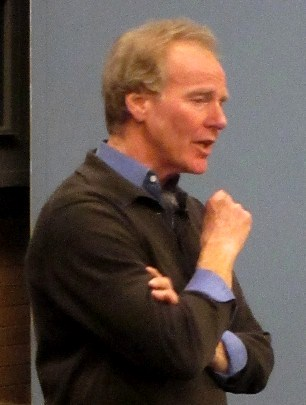
\includegraphics[height=3.3cm]{Peter_Senge_at_Quest_to_Learn.jpg}
		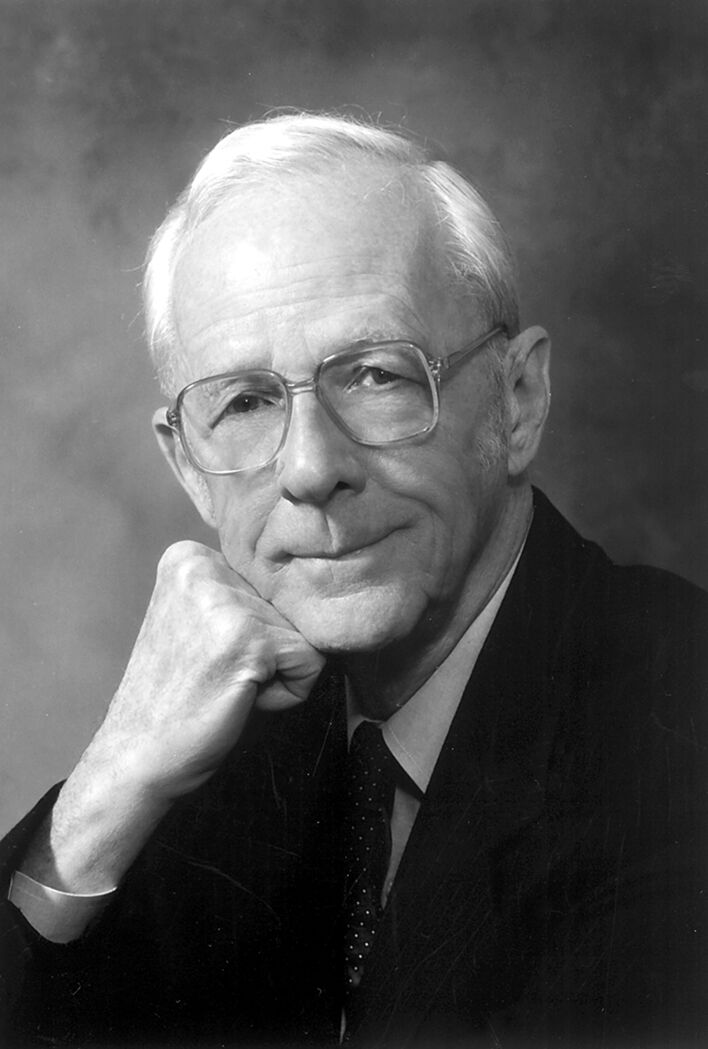
\includegraphics[height=3.3cm]{jayforrester.jpg}
		\caption{Peter Senge\index{Senge, Peter} (By Beyond My Ken - Own work, GFDL, \url{https://commons.wikimedia.org/w/index.php?curid=24627572}) ja Jay Forrester\index{Forrester, Jay}}
		\label{fig:legendid}
	\end{center}
\end{marginfigure}


\begin{marginfigure}
	\begin{center}
		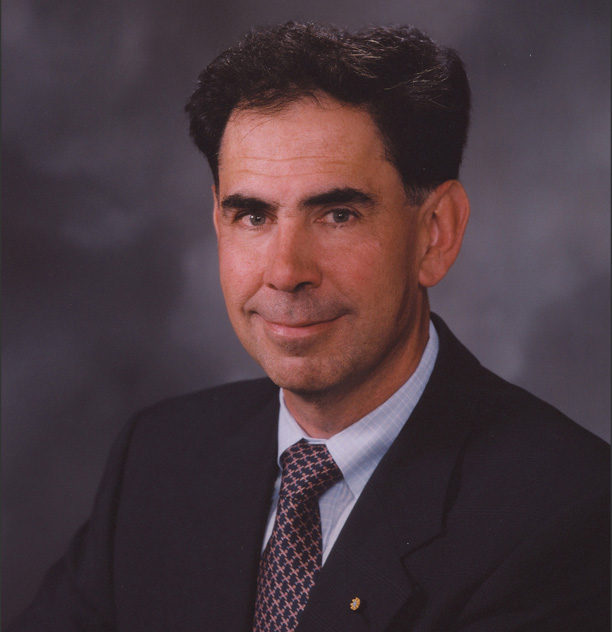
\includegraphics[height=3.3cm]{MIT-Ed-Crawley_0.jpg}
		\caption{Edward Crawley}
		\label{fig:ed}
	\end{center}
	Kauaaegne MIT professor Ed Crawley\index{Crawley, Edward} on töötanud koos NASAga ISSi kallal, asutanud mitmeid ettevõtteid ning olnud Skoltechi esimene rektor. Prof. Crawley süsteemiarhitektuuri üks vaieldamatuid suurkujusid maailmas.
\end{marginfigure}

Edward Crawley defineerib süsteemi arhitektuuri\index{Süsteem!Arhitektuur}\index{Arhitektuur!Definitsioon} nii:
\quote{The embodiment of concept, and the allocation of physical/informational function to elements of form, and definition of interfaces among the elements and with the surrounding context.}

Vaadakem seda definitsiooni lähemalt. 

Esmalt rõhtutatakse kontseptsiooni mõistet. Kontpsetsioon\index{Kontseptsioon!Definitsioon} on süsteemi peamine mõttemudel ja lähenemisviis, mis seob funktsiooni just selle konkreetse lahendusega. On tähenduslik, et seda mainitakse esimesena: just see osis seob definitsiooni tervikuks olles samas ka mainitud mõistetest kõige hoomamatum. Funktsioon\index{Funktsioon!Definitsioon} on see, mida süsteem \emph{teeb}. Siit tuleneb süsteemi kasulikkus ja ta on teenitult paigutatud järgmisele kohale. Vorm\index{Vorm!Definitsioon} on see, mis süsteem \emph{on}. Siit tulenevad süsteemiga seotud kulud. Näeme, et süsteemi puhul on oluline kolmik vorm, funktsioon ja kontseptsioon ning et tegu on üldise definitsiooniga. Ei funktsiooni ega vormi kohta ei öelda muud, kui et neil on mingisugune sisemine struktuur. Järgnevalt mainitakse liideseid\index{Liidesed} elementide vahel. Ehk, süsteemi puhul on oluline ka viis, kuidas tema elemendid suhestuvad nii omavahel kui ka ümbritseva keskkonnaga.

\section{Printsiipidest}
\index{Arhitektuur!Printsiibid}
Arhitektuuriga süvitsi tegelemisel on hea mõte pidada printsiipide päevikut. Arhitektuuris on mõttemudelil oluline koht ja seega on mõistlik tegeleda oma isikliku mõttemudeli arendamise ning dokumenteerimisega. Printsiibipäevik on üks viis seda teha. Printsiip on miski, mis tundub kehtivat alati ning mis ei sõltu teistest. Teatavas mõttes on tegemist universaalse tõega. Üheks näiteks printsiipidest arvutivõrkude vallas on RFC 1925\cite{callon1996rfc}. Printsiibipäeviku mõte on selles, et iga kord, kui igapäevases töös tundub mõni printsiip silma jäävat, kirjutatakse see jalamaid üles. Perioodiliselt vaadatakse päevik üle lootuses destilleerida kirja pandust veel universaalsemaid ja üldisemaid põhimõtteid. Üks näide sellisest päevikust on \cite{archprinciples}. 

Arhitektuuri printsiipide osas tuleb jälle viidata \citeauthor{crawley2015systems} tööle. Ta peab printsiipe nii oluliseks teadmuse jagamise vahendiks, et on need paigutanud raamatu sisekaanele. Üheks näiteks tema printsiipidest on arhitekti rolli printsiip \enquote{Arhitekti roll on vähendada ebamäärasust, fokusseerida loovust ja vähendada keerukust}\cite{crawley2015systems}.

\section{Emergentsusest}
Ingliskeelsel terminil \emph{emergence}\index{Emergents} on eesti keeles vasteks emergentsus\footnote{Vahel öeldakse ka ``ilmnemine``: Emergent behaviour tõlgitakse kui \enquote{ilmnev käitumine}}. Nii tähistatakse süsteemi omadust, mis seisneb millegi ilmnemises tänu mingitele muudele süsteemi omadustele. Arhitektuuri kontekstis on emergentsus süsteemide omadus lisaks disaini kaudu eesmärgiks seatud omadustele ka teiste omaduste ilmnemiseks. Tüüpiline emergentne omadus on võime inimesi tappa: suur hulk tehnoloogiaid alates tulest ja lõpetades tuumareaktsiooniga on mingil hetkel osutunud efektiivseks vaenlastest vabanemise vahendiks. Esimene nuga ei olnud mõledud mõrvaks kuid seda on nii aegade algusest kasutatud. Tüüpiliselt ei ole probleem mitte niivõrd süsteemi enda emergentsed omadused vaid emergents, mis sünnib eri objektide kombinatsioonist. Laua funktsioon on toetada asju. Joonlaua funktsioon on sirgeid jooni tõmmata. Kui aga asetada joonlaud poolenisti lauale, oleme saanud, sõltuvalt vaatepunktist, kas muusikariista või inimeste ärritamise vahendi. 

Mitte kõik emergentsed omadused ei ole lihtsalt ebasoovitavad või ootamatud \cite{emergence} toob häid näiteid sellest, kuidas pilvelõhkujad oma arhitektuuriga lausa inimesi ohustada võivad.

\section{Süsteemi piiride probleem}
\label{sec:boundary}
\index{Süsteem!Piirid}
Kui rääkida süsteemist, tekib alati küsimus süsteemi piiridest: kus algab meie kontrolli all olev ala ja kus ta lõpeb? \cite{wood2013framework} räägib osapoolte kaasamisest ning probleemipüstituse juures küsib õigesti: kuidas saada kontrolli alla konkreetse rakenduse teise ja kolmanda järgu efektid? Ehk, kuidas vältida projekti ebaõnnestumist, sest temast tõusis kahju meie olulise kliendi olulisele partnerile? Lahendusteks pakutakse osapoolte omavaheliste suhete analüüsi sotsiaalvõrkude puhul kasutatavate meetoditega. Siiski ei anta ka siin vastust küsimusele kirjeldatud võrgu piiridest: ei ole selge, kuidas otsustatakse, keda võrku kaasata ja keda mitte (kas kliendi kliendi klient on ka oluline?). 

Lisaks konkreetsele osapoolte kaardistamise raamistikule annab artikkel ka mõningase ülevaate erinevatest EA raamistikest.

	
\section{Küsimusi aruteluks}
\subsection{Millist väärtust loob arhitektuuriga tegelemine?}
Arhitektuur tundub oluline kuid samas on ka selge, et arhitekti mitteilmumine tööle ei põhjusta tavaliselt kohest kadu produktiivsuses. Arhitekti töö väärtust on mõnevõrra keeruline hinnata. 

Peamine sõnum auditooriumist: mõjuanalüüs, suur pilt, optimiseerimine/kulud
\TODO kirjuta lahti

\subsection{Kui palju erineb süsteemimõtlemisele tuginev mudel harjumuspärasest?}
Palju.
\TODO Näide testimise modelleerimisest. Lineaarne vs. mittelineaarne lähenemine

\section{Kirjuta lahti}
Arhiteketuuri ja organisatsiooni kooskõla. võrgustik-võrgustik Stella Soomlais studio case